\begin{filecontents*}[overwrite]{iac.cls}
%% iac.cls - IAC Conference Paper Class (2025)
%======================================================================================
%                                   CLASS CONFIGURATION
%======================================================================================
\NeedsTeXFormat{LaTeX2e}
\ProvidesClass{iac}[2025 IAC conference paper LaTeX class]

%--------------------------------------------------------------------------------------
% Options Handling
%--------------------------------------------------------------------------------------
\RequirePackage{kvoptions}
\DeclareStringOption[ieee]{bibstyle}        % Citation style
\DeclareStringOption[english]{language}     % Document language
\DeclareBoolOption{unicode}                 % Unicode support
\DeclareBoolOption{placeins}                % Float placement control
\ProcessKeyvalOptions*\relax

% Pass unknown options to article class
\DeclareOption*{\PassOptionsToClass{\CurrentOption}{article}}
\ProcessOptions\relax

%--------------------------------------------------------------------------------------
% Base Class and Geometry
%--------------------------------------------------------------------------------------
\LoadClass[twocolumn,letterpaper,10pt]{article}

\RequirePackage[
    margin=2.5cm,
    top=2.5cm,
    headsep=1cm,
    bottom=3.5cm
]{geometry}
\setlength{\columnsep}{0.5cm}

% Footer positioning calculation
\setlength{\footskip}{
    \dimexpr
        (\paperheight - 
            (1in + \voffset + \topmargin + \headheight + \headsep + \textheight)
        ) - 1.5cm
}

%======================================================================================
%                                PACKAGE CONFIGURATION
%======================================================================================
\RequirePackage{etoolbox}                               
\RequirePackage{xcolor}                                 
\RequirePackage{graphicx}                               
\RequirePackage{booktabs}                               
\RequirePackage{fancyhdr}                               
\RequirePackage{lastpage}                               
\RequirePackage[explicit,compact]{titlesec}             
\RequirePackage{alphalph}                               
\RequirePackage{caption}                                
\RequirePackage{fmtcount}                               
\RequirePackage{contour}                                
\RequirePackage[normalem]{ulem}
\RequirePackage{float}                                  
\RequirePackage{microtype}                              
% Math support
\RequirePackage{amsmath,amssymb,amstext,amsfonts,bm}
% Math structures
\RequirePackage{array,empheq,amsthm,thmtools}                               
% Scientific notation
\RequirePackage{siunitx}                                
\sisetup{detect-all}
\RequirePackage[version=4]{mhchem}
\RequirePackage{extarrows,gensymb,latexsym,optidef}                                
% Hyperlinks and references
\RequirePackage[colorlinks=false,allcolors=blue,unicode=true]{hyperref}
\RequirePackage{xurl}                                   
% Bibliography
\RequirePackage[backend=biber,style=\iac@bibstyle,citestyle=numeric-comp]{biblatex}
\RequirePackage[capitalise]{cleveref}                   
\RequirePackage{csquotes}                               
\RequirePackage[bottom]{footmisc}                       
\RequirePackage{enotez}

%======================================================================================
%                                TEXT FORMATTING
%======================================================================================
% Cross-reference formatting
\renewcommand*{\sectionautorefname}{Section}
\renewcommand*{\subsectionautorefname}{Subsection}
\renewcommand*{\subsubsectionautorefname}{Subsection}
\renewcommand*{\equationautorefname}{Eq.}
\renewcommand*{\figureautorefname}{Fig.}
\renewcommand*{\tableautorefname}{Table}
\providecommand*{\listingautorefname}{Listing}

% Caption formatting
\captionsetup[figure]{name=Fig.,format=hang,indention=-20pt,labelsep=period}
\captionsetup[table]{format=hang,indention=-24pt,labelsep=period}

%======================================================================================
%                                TYPESETTING SETTINGS
%======================================================================================
% Font configuration
\RequirePackage{fontspec}
\setmainfont{TeX Gyre Termes}

% Section formatting
\titleformat{\section}{\normalfont\bfseries}{\arabic{section}.~}{0pt}{#1}
\titleformat{\subsection}{\normalfont\itshape}{\arabic{section}.\arabic{subsection}~}{0pt}{#1}
\titleformat{\subsubsection}{\normalfont\itshape}{\arabic{section}.\arabic{subsection}.\arabic{subsubsection}~}{0pt}{#1}

% Table enhancements
\newcommand{\thickhline}{\noalign{\ifnum 0=`}\fi \hrule height 2pt \futurelet \reserved@a \@xhline}
\newcolumntype{"}{@{\hskip\tabcolsep\vrule width 1pt\hskip\tabcolsep}}

% Footnote symbols
\newcommand*{\fnsymbolsingle}[1]{\ensuremath{\ifcase#1\or *\or \dagger\or \ddagger\or \mathsection\or \mathparagraph\else\@ctrerr\fi}}
\newalphalph{\fnsymbolmult}[mult]{\fnsymbolsingle}{}
\renewcommand*{\thefootnote}{\fnsymbolmult{\value{footnote}}}
\def\tagform@#1{\maketag@@@{[#1]\@@italiccorr}}

% URL formatting
\renewcommand\UrlFont{\ttfamily}

% Underline styling
\renewcommand{\ULdepth}{1.8pt}
\contourlength{0.8pt}
\let\@uline\uline
\renewcommand{\uline}[1]{\@uline{\phantom{#1}}\llap{\contour{white}{#1}}}

% Ordinal numbers
\newcommand{\nth}[1]{\ordinalnum{#1}}

% Year shorthand
\newcommand*{\yearshorthand}[1]{\expandafter\@gobbletwo\number\numexpr#1\relax}

%======================================================================================
%                                MATHEMATICS SETTINGS
%======================================================================================
\let\@forall\forall
\renewcommand{\forall}{\ensuremath{\,\@forall\,}}
\DeclareRobustCommand{\vect}[1]{\vec{#1}}
\renewcommand*{\qed}{\quad\square}
\newcommand{\indep}{\ensuremath{\perp\!\!\!\perp}}
\mathchardef\mathmul=\mathcode`*
\mathcode`*=\cdot
\DeclareMathOperator{\E}{\mathbb{E}}
\DeclareMathOperator{\prob}{p}
\DeclareMathOperator{\tr}{tr}
\DeclareMathOperator{\diff}{\mathop{}\!{d}}
\DeclareMathOperator{\conv}{\ast}

% Adjust spacing around equations
\g@addto@macro\normalsize{%
  \setlength\abovedisplayskip{2.5pt}%
  \setlength\belowdisplayskip{7.5pt}%
  \setlength\abovedisplayshortskip{2.5pt}%
  \setlength\belowdisplayshortskip{7.5pt}%
}

%======================================================================================
%                                iac-SPECIFIC ELEMENTS
%======================================================================================
% Author tracking
\newcounter{authcount}
\newcounter{contactauthor}
\NewDocumentCommand{\authoriac}{ s m m m }{%
    \stepcounter{authcount}%
    \csdef{iac@author\theauthcount}{#2}%
    \csdef{iac@affiliation\theauthcount}{#3}%
    \csdef{iac@email\theauthcount}{#4}%
    \IfBooleanT{#1}{\setcounter{contactauthor}{\theauthcount}}%
}

% Abstract formatting
\renewcommand{\abstract}[1]{%
    \def\iac@abstract{%
        \vspace*{-2em}%
        \begin{center}\bfseries Abstract\end{center}%
        \vspace*{-0.8em}%
        \setlength{\parindent}{0.5cm}%
        \setlength{\parskip}{0pt}%
        #1%
    }%
}

% Conference metadata
\newcommand*{\ConfInfo}[1]{\def\iac@conference{#1}}\ConfInfo{}
\newcommand*{\ConfLoc}[1]{\def\iac@location{#1}}\ConfLoc{}
\newcommand*{\dateofiac}[1]{\def\iac@dates{#1}}\dateofiac{}
\newcommand*{\yearofiac}[1]{\def\iac@year{#1}}\yearofiac{}
\newcommand*{\Papernumber}[1]{\def\iac@papernumber{#1}}\Papernumber{}
\newcommand{\copyrightIAFIAC}[2]{\def\iac@copyright{Copyright \copyright\,#1 by #2. All rights reserved.}}

%======================================================================================
%                                PAGE DESIGN
%======================================================================================
% Paragraph indentation
\setlength\parindent{0.5cm}

% Section spacing
\titlespacing{\section}{0pt}{1em plus 0.5em}{0pt}
\titlespacing{\subsection}{0pt}{1em plus 0.5em}{0pt}
\titlespacing{\subsubsection}{0pt}{1em plus 0.5em}{0pt}

% Header/footer configuration
\fancypagestyle{fancy}{%
    \chead{{\footnotesize\color{gray}%
        International~Astronautical~Congress~(IAC 2025),~\iac@location,~\iac@dates~\iac@year.\\%
        \iac@copyright%
    }}%
    \lhead{}%
    \rhead{}%
    \renewcommand{\headrulewidth}{0pt}%
    \lfoot{{\color{gray}iac--\yearshorthand{\iac@year}--\iac@papernumber}}%
    \cfoot{}%
    \rfoot{{\color{gray}Page \thepage\ of \pageref{LastPage}}}%
}
\pagestyle{fancy}

% Title page layout
\renewcommand\maketitle{\twocolumn[
    \begin{@twocolumnfalse}
        \begingroup
            \global\@topnum\z@
            \@maketitle
            \@thanks
        \endgroup
    \end{@twocolumnfalse}
]}

% Title formatting
\def\@maketitle{%
    {\centering%
        iac--\yearshorthand{\iac@year}--\iac@papernumber\par%
        \vskip1em
        {\bfseries\selectfont \@title \par}%
        \vskip 1em%
        \begin{center}%
            \lineskip .5em%
            \newcounter{authnum}%
            \setcounter{authnum}{0}
            \whileboolexpr{ test {\ifnumcomp{\value{authnum}}{<}{\theauthcount}} }{%
                \stepcounter{authnum}%
                \mbox{%
                    \normalfont\textbf{\csuse{iac@author\theauthnum}\textsuperscript{\alph{authnum}}}%
                    \ifboolexpr{ test {\ifnumcomp{\value{authnum}}{=}{\thecontactauthor}} }%
                        {\textsuperscript{\kern-1pt$\conv$}}{}%
                    \ifboolexpr{ test {\ifnumcomp{\value{authnum}}{<}{\theauthcount}} }{,~}{}%
                }%
            }%
        \end{center}%
    }%
    {\small\itshape\selectfont%
        \setcounter{authnum}{0}
        \whileboolexpr{ test {\ifnumcomp{\value{authnum}}{<}{\theauthcount}} }{%
            \stepcounter{authnum}%
            \parbox{0.75em}{\normalfont\textsuperscript{\alph{authnum}}}\csuse{iac@affiliation\theauthnum},~\uline{\csuse{iac@email\theauthnum}}\par
        }%
        \parbox{0.75em}{\textsuperscript{*}}Corresponding author
    }%
    \vskip 1em%
    \indent\iac@abstract\par%
    \vskip 4.5ex
}
\end{filecontents*}

%======================================================================================
%                                MAIN DOCUMENT
%======================================================================================
\documentclass{iac}
\addbibresource{references.bib}

\begin{document}

% Conference metadata
\ConfInfo{4}
\ConfLoc{Sydney, Australia}
\dateofiac{14-18 October}
\yearofiac{2025}
\Papernumber{15-1.2.3}
\copyrightIAFIAC{2025}{the International Astronautical Federation (IAF)}

% Title and authors
\title{Manuscript Template and Style Guide (Title of Your Paper)}
\authoriac*{Eva Y.-W. Chang}
           {Department of Tourism and Hospitality, China University of Science and Technology, 200 Chunghwa Street, Henshan Village, Hsinchu County, Taiwan 31241}
           {}
\authoriac{Rock J.-S. Chern}
          {Department of Aerospace Engineering, Ryerson University, 350 Victoria Street, Toronto, Ontario, Canada M5B 2K3}
          {}

% Abstract
\abstract{A concise and factual abstract (written in third person and in one paragraph) of no more than 400 words is required. The abstract should state briefly the purpose of the research, the principal results and major conclusions. An abstract must be stand alone and complete in itself with no references to the main body of the manuscript. References should be avoided, but if essential, then cite the author(s) and year(s). Also, non-standard or uncommon abbreviations should be avoided, but if essential they must be defined at their first mention in the abstract itself. Readers should not have to read the full text to understand the abstract. The abstract can be an updated version of the one submitted at the call-for-abstracts, but its contents must not differ substantially.
\\\textbf{Keywords}: (Maximum 6)
}

\maketitle

% Document sections
\section*{Nomenclature}
This section is not numbered. A nomenclature section could be provided when there are mathematical symbols in your paper. Superscripts and subscripts must be listed separately. Nomenclature definitions should not appear again in the text.

\section*{Acronyms/Abbreviations}
This section is not numbered. Define acronyms and abbreviations that are not standard in this section. Such acronyms and abbreviations that are unavoidable in the abstract must be defined at their first mention there. Ensure consistency of abbreviations throughout the article. Always use the full title followed by the acronym (abbreviation) to be used, e.g., reusable suborbital launch vehicle (RSLV), International Space Station (ISS).

\section{Introduction}
Section headings are in \textbf{bold} and placed flush on the left hand margin of the column. The Introduction Section is to state the objectives of the work, provide an adequate background including a brief literature survey, major differences from the others, and sectional organization of this paper. Avoid a too detailed and lengthy literature survey and a summary of the results.

Divide your paper into clearly defined and numbered sections numbered 1., 2., …. Subsections should be numbered 1.1 (then 1.1.1, 1.1.2, ...), 1.2, etc. Use this numbering also for internal cross-referencing: do not just refer to “the text”. Any subsection may be given a brief heading. Each heading should appear on its own separate line.

\subsection{Subsection headings}
Subsection headings are in italics and placed flush on the left hand margin of the column.

\subsubsection{Sub-subsection headings}
Sub-subsection headings are in italics and placed flush on the left hand margin of the column.

\section{Materials and methods}
Provide sufficient detail to allow the work to be reproduced. Methods already published should be indicated by a reference: only relevant modifications should be described.

\section{Theory and calculation}
A Theory section should extend, not repeat, the background to the article already dealt with in the Introduction and lay the foundation for further work. In contrast, a Calculation section represents a practical development from a theoretical basis.

\subsection{Equation numbers}
Number consecutively any equations that have to be displayed separately from the text (if referred to explicitly in the text). The numbers identifying the equations should be placed in parentheses to the right of the equation. For example:
\begin{equation}
    \vect{F}_g = -G\frac{m*m_E}{R_E^2}\vect{i}_r = m\vect{g}_{ta}
\end{equation}

\subsection{Figure numbers}
Ensure that each figure/illustration has a title. All figures/illustrations must be numbered and cited (see \autoref{fig:SpaceShipTwo carried under White Knight Two}) in the text consecutively. Place figures/ illustrations as close as possible to the first references to them in the manuscript. Restrict them to single-column width unless this would make them illegible (then extend these figures/illustrations across two columns or place them to the end of your paper).

\begin{figure}[H]
    \centering
    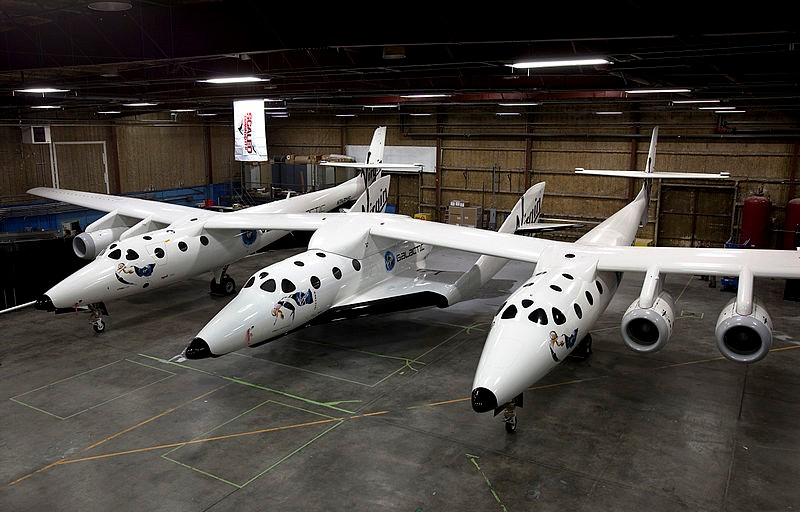
\includegraphics[width=0.8\linewidth]{figures/SpaceShipTwo.jpg}
    \caption{SpaceShipTwo carried under White Knight Two}
    \label{fig:SpaceShipTwo carried under White Knight Two}
\end{figure}

\subsection{Tables}
Tables can be placed either next to the relevant text in the article, or on separate page(s) at the end. Number and cite (as shown in \autoref{tab:Major data of the orbits of Venus, Earth, Mars and Jupiter}) tables consecutively in accordance with their appearance in the text. Place table title above and any remarks below the table body.

\begin{table}[H]
\caption{Major data of the orbits of Venus, Earth, Mars and Jupiter}
\label{tab:Major data of the orbits of Venus, Earth, Mars and Jupiter}
\centering
\begin{tabular}{lllll}
\thickhline
           & Venus   & Earth & Mars  & Jupiter \\ \hline
M/ME       & 0.82    & 1     & 0.11  & 317.89  \\ 
e          & 0.007   & 0.017 & 0.093 & 0.048   \\
R (AU*)    & 0.7233  & 1     & 1.524 & 5.203   \\
i (deg)    & 3.40    & 0     & 1.85  & 1.30    \\
T (years)  & 0.62    & 1     & 1.88  & 11.86   \\ \thickhline
\multicolumn{5}{l}{* AU =   Astronomical Unit}
\end{tabular}
\end{table}

Tables with a moderate amount of information should be positioned within one column. Tables, figures or pictures with large amounts of information or size may extend across two columns.

\subsection{Page numbers}
Indicate page number at the bottom of each page.

\section{Results}
Results should be clear and concise.

\section{Discussion}
This should explore the significance of the results of the work, not repeat them. A combined Results and Discussion section is often appropriate. Avoid extensive citations and discussion of published literature.

\section{Conclusions}
The main conclusions of the study may be presented in a short Conclusions section, which may stand alone or form a subsection of a Discussion or Results and Discussion section.

\section*{Acknowledgements}
This section is not numbered.

\section*{Appendix A (Title)}
This section is not numbered.

\section*{Appendix B (Title)}
This section is not numbered.

\section*{Etc.}
This section is not numbered.

\section*{References}
\subsection*{In the text}
Indicate references by number(s) in square brackets in line with the text. The actual authors can be referred to, but the reference number(s) must always be given.

\subsection*{List of references}
Example: “..... as demonstrated \cite{geer2010art,chang2015space,strunk2000elements,mettam2009prepare}. Mack \cite{mack2015virgin} obtained a different result ....”

\printbibliography[heading=none]

\end{document}